The controls layer is responsible for binding all modules of the Turing Board to be part of the same system. All data coming in is intercepted by this layer and forwarded to the respective modules which are responsible for processing the forwarded data.

\subsection{Layer Hardware}
The hardware involved in this layer consists of the following:
\begin{itemize}
    \item Nvidia Jetson TX2 responsible for running the controls code.
    \item VESC responsible for the speed control of the wheels.
    \item Intel real sense camera responsible for capturing real time footage for the follow-me feature and autonomous navigation.
    \item Texas Instruments Tiva C Series microcontroller which controls the turning mechanism.
\end{itemize}

\subsection{Layer Operating System}
The Layer makes use of the Linux operating system to run applications such as the control code.

\subsection{Layer Software Dependencies}
\begin{itemize}
    \item Python Dependencies
    \begin{itemize}
        \item PyVESC
        \item Pyrebase
        \item Pyserial
        \item Pycrc
        \item Threading
    \end{itemize}
\end{itemize}

\subsection{Controls Subsystem}
There are three main components of project which calls for this piece of software which must all be non-blocking in nature to ensure the entire system stays responsive.
\begin{itemize}
    \item Reading data from the microcontroller.
    \item Forwarding data to the microcontroller.
    \item Fetching data from the Firebase Real-time database.
\end{itemize}

\begin{figure}[h!]
	\centering
 	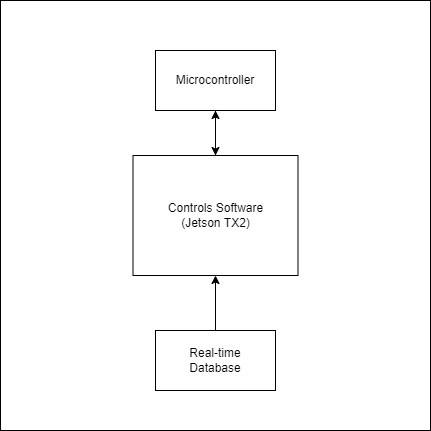
\includegraphics[width=0.60\textwidth]{images/Controls Software Subsystem.drawio.png}
 \caption{Example subsystem description diagram}
\end{figure}

\subsubsection{Subsystem Hardware}
The controls subsystem does not consist of explicit hardware. All work is done through software to communicate information.

\subsubsection{Subsystem Operating System}
The controls subsystem does not make use of an underlying operating system. The layer makes use of the Linux operating system.

\subsubsection{Subsystem Software Dependencies}
\begin{itemize}
    \item Python Dependencies
    \begin{itemize}
        \item PyVESC
        \item Pyrebase
        \item Pyserial
        \item Pycrc
        \item Threading
    \end{itemize}
\end{itemize}

\subsubsection{Subsystem Programming Languages}
\begin{itemize}
    \item Python
    \begin{itemize}
        \item Used for the main controls system.
    \end{itemize}
    \item C
    \begin{itemize}
        \item Used to program the microcontroller.
    \end{itemize}
\end{itemize}

\subsubsection{Subsystem Data Structures}
\begin{itemize}
    \item Classes
    \begin{itemize}
        \item Controls
        \begin{itemize}
            \item Responsible for running the controls code.
        \end{itemize}
        \item SerialCommunication
        \begin{itemize}
            \item Establishes connection with the microcontroller.
        \end{itemize}
    \end{itemize}
\end{itemize}

\subsubsection{Subsystem Data Processing}
After fetching data from the database, the controls software will process the data first to an extent. Since data coming in will be floating point values, it first needs to be translated into value which the microcontroller can understand. So, the entire range of data from the remote control app is taken and the required data is mapped from 0-255 which is then forwarded to the microcontroller which causes the wheels to change speed. As part of the same data packet, angle data from the controls code is also sent to the microcontroller which aids in turning the turning mechanism to a specific angle with respect to the turning mechanisms origin. Any data such as weight values if someone is standing on the long board (an integral part of the design so that the software knows when to turn off the turning mechanism) is received back in the same data format (0-255) which gets translated to weight values inside of the controls code.